\documentclass[a4paper,10pt,oneside]{book}
\usepackage[table,xcdraw]{xcolor}
\usepackage{graphicx}
\usepackage{float}
\usepackage{hyperref}
\usepackage[T1]{fontenc}
\usepackage{mathptmx}
\usepackage[utf8]{inputenc}
\usepackage{setspace}
\usepackage[paper=a4paper,margin=1in]{geometry}
\usepackage{imakeidx}
\usepackage{tikz}
\usepackage{fancyvrb}
\usepackage{amssymb}% http://ctan.org/pkg/amssymb
\usepackage{pifont}% http://ctan.org/pkg/pifont
\newcommand{\cmark}{\ding{51}}%
\newcommand{\xmark}{\ding{55}}%
\usepackage{caption}
\usetikzlibrary{positioning, quotes}
\usepackage[english]{babel}
\usepackage[skip=10pt plus1pt, indent=40pt]{parskip}
\usepackage[
  backend=bibtex,
  style=numeric,
  sorting=ydnt
  ]{biblatex}
\addbibresource{quotes.bib}
\makeindex

\newcommand{\putimage}[3] {
	\begin{figure}[H]
	    \centering
	    \includegraphics[width=0.9\linewidth]{#1}
	    \caption{#2}\label{#3}
	\end{figure}
}

\begin{document}
    
    \begin{titlepage}
        
        \noindent
        \begin{minipage}[t]{0.19\textwidth}
            \vspace{-4mm}{
\includegraphics[scale=1.15]{logo_unimib.pdf}}
        \end{minipage}
        \begin{minipage}[t]{0.81\textwidth}
        {
                \setstretch{1.42}
                {\textsc{Università degli Studi di Milano - Bicocca}} \\
                \textbf{Scuola di Scienze} \\
                \textbf{Dipartimento di Informatica, Sistemistica e Comunicazione} \\
                \textbf{Master Degree in Computer Science} \\
                \par
        }
        \end{minipage}
        
	\vspace{40mm}
        
	\begin{center}
            {\LARGE{
                    \setstretch{1.2}
                    \textbf{Failing to solve traffic with Reinforcement Learning and Curriculum approaches}
                    \par
            }}
            {\large{
                    \setstretch{1.2}
                    \textit{What is SUMO and why intelligent traffic lights would make traffic worse}
                    \par
            }}
        \end{center}
        
        \vspace{50mm}

        \noindent
        {\large \textbf{Supervisor:} Prof. Giuseppe Vizzari}
        
        \vspace{15mm}

        \begin{flushright}
            {\large \textbf{Candidate:}} \\
            \large{Refolli Francesco} \\
            \large{Matricola 865955} 
        \end{flushright}
        
        \vspace{40mm}
        \begin{center}
            {\large{\bf Academic Year 2024-2025}}
        \end{center}

        \restoregeometry
        
    \end{titlepage}

    \begin{abstract}

This thesis investigates the effectiveness of curriculum learning approaches for modular training processes as alternative to monolithic (exhaustive) experience generation processes, compares tabular reinforcement learning methods to deep reinforcement learning models, evaluates the benefits of learning agents as opposed to fixed cycle traffic light programs, analyzing sensitivity of key hyperparameters such as the number of quantization levels for state space discretization, evaluates the advantages given by multi agent learning techniques, which involves sharing observations and rewards among agents, and finally determines whether a self-adaptive algorithm is able to update and correct the agent over time to make up for performances degrading over time due to demand and infrastructure changes.
A fork of the SUMO-RL framework, a bridge between SUMO (Simulator of Urban MObility) and Python which provides an integrated environment for developing and running reinforcement learning models, has been developed in order to answer the aforementioned research objectives,  enhancing its performance and capabilities, implementing new agents and observation/reward functions, allowing agents to share slices of observations/rewards and adding a self-adaptive algorithm for learning on degrading performances. Experiments are executed with the computational resources provided by hpc-ReGAInS@DISCo, which is a MUR Department of Excellence Project within the Department of Informatics, Systems and Communication at the University of Milan-Bicocca.

\end{abstract}

    \printindex
    \tableofcontents
    \renewcommand{\baselinestretch}{1.5} 

    \chapter{Traffic Science}

\section{Introduction}

\paragraph{Terminology}

In the rest of the document we will refer to \textit{transit} or \textit{flow} to indicate a group of traveling vehicles.
The word \textit{traffic} will be used only indicate the phenomenon of high density flows where there is the perception of being slowed down.
The word \textit{jam} will indicate strictly a deadlock traffic event.

\paragraph{Vehicles}

This is a umbrella term for referring to any kind of entity which travels along a network.
Vehicles \textbf{can} have an \textit{origin} and a \textit{destination}: for example, private motor vehicles are usually driven in order to go from a \textit{point-of-interest} A to a point point-of-interest B.
An interesting exception are those public transit vehicles serving on a \textit{circle line} like the M3 City Circle Line of Copenhagen, and in general vehicles offering public transit logically have more than one destination while carrying out a trip.
Vehicles attempt to follow a \textit{desired path}, which is influenced by various factors: network knowledge, habits, transit regulations and so on.
This path can diverge from the \textit{actual path} they end up following for various reasons: accidents, infrastructure works, events and maybe illegal parking.
A notable exception are fixed route vehicles (such as public transit) and in particular track-constrained vehicles (such as trams and trains).
In both cases, the whole journey is not required to be completed: a vehicle can override its route because of change of heart (the case of private vehicles), rescheduling (the case of public transit) or else.
Depending on the goal of a simulation, the flow can be restricted to a small set of vehicle types, but in the real world, the vehicle flow can be heterogeneous: cars, trolleybuses, trams, emergency vehicles, trucks, bicycles, motorbikes and so on. Each vehicle has different physical properties and different allowances.
Vehicles allowance rules can be defined by diving the flow with respect to origin/destination, vehicle type (cars \textit{mustn't} ride in bike lanes), local regulations (in some cities, taxis \textit{may} use public transit lanes), vehicle properties (\textit{only} motor vehicles able to reach at least 60 km/h can drive on the motorway) or even driver properties (\textit{limited traffic zones} are open only for residents).
This partitioning activity is a form of transit regulation and characterizing vehicles by their properties rather than transparent objects helps (TODO: CITAZIONE) in managing their transit, resolving path conflicts and also enhancing the quality of life of residents (a bypass \textit{should} cut a significant amount of transit vehicles in city centers).

\paragraph{Infrastructure}

The road network can be represented with a \textbf{directed multi-graph} of intersections and roads. Each road has one or more lanes, a maximum speed and vehicles allowances dictating which kind of vehicles are allowed to flow through it. While more simplistic models use undirected graph with labelled edges to represent lanes and one/two-way traffic, it should be noted that a simple directed graph wouldn't be sufficient as in real-world road networks the may be more different links between an intersection. While some network slices could be represented with a single edge, there are more complex situations as in figure \ref{fig:multigraph-is-better-than-nothing} (a slice of Viale Zara, Milan, Italy) in which two big intersections are linked with two main one-way three-lane roads, two side one-way one-lane roads ("controviali") and two dedicated links for tramway vehicles. These roads are physically separated with median strips and each link may allow for different turns within the intersections. Of course, the implementation model can be optimized for performance, but the logical model should remain a multi-graph because it better represents the features of the road network.

\paragraph{Traffic}

\textbf{Traffic} can be defined as a flow of vehicles on a network with peaks of density in some locations in which the average speed of those vehicles is significantly lower than the average of the entire network.
Mathematically speaking, \textbf{traffic} emerges when many vehicles need or want to transit through a shared path which hasn't enough capacity for handling this high number of users.
Urban planning authorities have since then taken this hint quite literally, adding lanes year-by-year, but in the end the only result was an increase in the number of road vehicles with unchanged transit density or, even worse, with higher travel times \cite{Speck2018}.
In this context, \textbf{traffic science} comes in help: it seeks to understand the causes of traffic as a social \textit{phenomenon} modeling demand and analyzing flaws and strengths of infrastructure.

In the following sections I'll explain and analyze the impact of some strategies for transit regulation and traffic reduction. I'll introduce the concepts of demand modeling. Finally I'll explain the main assumptions for the present simulation and present the scenarios being used.

\section{Transit Regulation}

All the strategies presented in this section involve the usage of infrastructure artifacts in order to optimize transit. The first group aims to manage excessive flows by organizing them into different streams by origin, destination or mean of transportation and modifying the road infrastructure. The second aims to reduce route conflicts and optimize the usage of intersections. None of those is able to "fix" traffic, there are no silver bullets. This section is intended to introduce the reader to the context of transit regulation.

\subsection{Managing high flows}

\paragraph{Just one more lane}

What happens when among all the route that can be possibly be followed there is one which is faster and more convenient? Different streams are going to merge into a single huge flow which is slower than the other ones. A reasonable but ineffective action is to increase the number of lanes \ref{fig:atlanta-georgia-freeway}, but that adds only capacity to the system. It temporally fluidify traffic until other vehicles arrive into the system because it has become more convenient than their current route, and eventually traffic reemerges.

\paragraph{Bypasses, freeways, motorways}

Freeways and motorways are an example of \textit{specialized roads} which can be used to segregate the flows of vehicles needing to travel long distances from the local/regional transit. Those are generally built far from urban areas and those are what prevented urban planners from extending local roads into ten-lanes wide monsters. A further example of specialized road are bypasses, which are used to cut travel times and reduce the number of vehicles that go through the city center, but can also be used in combination with motorways. For example, in image \ref{fig:bologna-bypass} are reported three alternatives proposed by authorities to build a bypass in the Bologna's motorway node to split the flow on the basis of whether those vehicles are going to Bologna or need to reach other destinations like Firenze and Ancona. Specialized roads are generally effective in reducing travel times and represent the more convenient way for traveling mid/long distances, however they require extensive land usage and are subject to increased demand. As they essentially only add capacity to the system, it's only a matter of time before vehicle density reaches jamming levels.

\paragraph{Transit zones}

The urban area can be divided into \textit{zones} in which some vehicles can or cannot enter with various kind of rules.
\textit{Restricted traffic zones} (\textbf{ZTL}) are effectively used in city centers to block the entrance of non-resident vehicles and reduce the number of vehicles in the area. Vehicles violating this blockage are subject to a fine. If this fine is too low or if the coverage is limited, the ZTL has the same effects of a CAS.
\textit{Controlled access zones} (\textbf{CAS}) are similar but only require the payment of a toll in order to enter in the zone. An infamous example is the Area C of the city of Milan, where in order to enter it, the driver needs to buy a ticket (but some vehicles are exempts). Usually, the toll is used as a deterrent for persuading drivers to avoid central areas. Unfortunately, this measure is usually misunderstood as a way of taxing non-residents or citizens.
Finally, in \textit{Low emission zones} (\textbf{LEZ}) the only vehicles which entrance is forbidden are the ones exceeding pollution limits (e.g. by Europe emission standards). This measure is effective only in those societies where electric vehicles (EVs) and low-emission vehicles make up a small percentage of registered vehicles, because otherwise a large number of vehicles would not be affected by this regulation.
In general, the more restrictive an area is and the more area it coverts, the more it reduces traffic and wear and tear of the road network. Nonetheless, zones can also have the side effect of increasing traffic in peripheral areas or citizen rage if the restricted area is not well served by public transit, if the are no interchange parking lots outside of the area and if it's not reachable by other means, such as buses and trains.

\paragraph{Dedicated lanes}

An effective way of cutting travel times and increasing security of vehicles traveling in a mixed network (this is the case of European cities), is drawing \textit{dedicated lanes} for public transit, bikes and pedestrians. In some cities also taxis are allowed to use public transit lanes and if the number of taxis in service is high, it ends up lowering the performance of dedicated lanes. However, cities are limited in space: dedicated lanes mean cutting the number of lanes for use of private vehicles, which take up most of the spaces in urban areas. Urban planners face opposition when cutting the space allocated to cars, so it is vital that such infrastructures are enforces and designed properly in order to satisfy the transit needs of replaced vehicles.

\paragraph{One-way roads}

Where space isn't enough for two-way roads with dedicated lanes, often a good solution is the implementation of one-way roads, which also lead to safer crossings and more manageable flows. This measure actually increases travel times of vehicles, which could induce some private vehicle passengers/drivers to travel with mass public transit or by bicycle, which ultimately can decrease mean travel time of all the users of the network.

\subsection{Managing conflicts}

\paragraph{Cloverleafs}

Intersections can be built in the form of \textit{cloverleafs} to remove entirely conflicts from crossing flows. While this offer high capacity and speed, it requires excessive land usage (as can be seen in figure \ref{fig:houston-interchange-siena}) and cannot be built in urban context without erasing entire neighborhoods.

\paragraph{Precedence rule}

In urban area, non regulated intersections often follow the precedence rule: a vehicle should wait for the transit of a vehicle coming from its right, for example. The clear advantage is the lack of specialized infrastructure, at the cost of dependency on human reaction times and some times it can lead to deadlocks.

\paragraph{Roundabouts}

In roundabouts, the precedence rule is "inverted": the precedence is given to vehicles which are already in the roundabout. Depending on reaction times, it is observed that it grants a continuous flow and minimizes idle times.

\paragraph{Traffic lights}

With respect to other regulation strategies, \textit{traffic lights} are more \textbf{interesting} since they offer flexibility and regulators can apply different programs over time.

\subparagraph{Fixed cycle}

The most common program is the \textit{fixed cycle program}. Every X seconds its state changes, switching from green to yellow and red, effectively selecting from which lanes vehicles are allowed to occupy the intersection and where they can go. An intuition is that with low cycle time (e.g. 10 seconds), the intersection behaves like a roundabout, which is advantageous when dealing with incoming traffic uniformly distributed among the entrances. With long cycles, the queue is less segmented (as start-and-stop phenomenon is reduced) but depending on the distribution of the incoming flows, it can lead to a waste of time, as vehicles from a trafficked main road may need to wait on red a long cycle with a deserted side road on green.

\subparagraph{Green-wave}

Traffic lights can be \textit{synchronized} in order to obtain a so-called \textit{green-wave}, in which many adjacent traffic lights are set to green in order to grant a continuous or uninterrupted flow. This can be achieved by directly synchronizing the phase of all traffic lights or by implementing a cycle schedule allowing groups of vehicles to flow in a direction while maintaining time separation with respect to preceding vehicles and vehicles from other directions crossing the intersections.

\subparagraph{Transit signal priority}

Precedence to tram and buses can be given by detecting their proximity to the traffic light regulated intersection. This drastically reduces waiting times for public transit vehicles, which eventually could reduce the number of circulating private vehicles and thus lower traffic levels. This can be applied also to other type of public vehicles like emergency vehicles.

\section{Demand models}

This section gives an introduction to demand modeling which will be useful in further chapters to explain how demand has been simulated and how scenarios have been created.
The two subsections answer two diffent aspects of demand modeling: space and time.

\subsection{Where?}

In \textit{Origin-destination matrices} (\textbf{OD Matrix}) every cell contains a number representing the approximate demand of transit vehicles from a zone A to a zone B. Depending of the scale of the simulation, zones can be regions, provinces, cities or urban districts.
For example, the Lombardy region yearly analyze traffic and demand \cite{ODLombardia2014} between its cities in order to plan maintenance and improvements in its regional road network.
It is useful that zones partition the area of interest without intersections, otherwise data could be distorted. This is often the case of urban contexts: for example Agenzia Mobilita' Ambiente e Territorio of Milan (AMAT) in 2010 \cite{ODMilano2010} had modeled the urban transit demand of the city of Milan but the zones used for OD matrix are not clearly distinguished (it can be seen in \ref{fig:odzones-milano-2010}) and therefore the matrix has to be taken with coarse-grain granularity.
Nonetheless, counting vehicles and inferring their origin destination it not an easy activity \cite{bell1983estimation}.

\subsection{When?}

Usually, mobility agencies create more than one OD matrix in order to capture how traffic levels change during a day.
Some agencies such as AMAT use three time ranges: 07:00-10:00 (morning peak), 10:00-16:00 (off-peak) and 16:00-20:00 (evening peak). 
While other entities like Regione Lombardia, provide hourly data.
In figures \ref{fig:odmatrix-milano-2010} and \ref{fig:odmatrix-lombardy-2014}, mean traffic levels from OD matrices of Milan and Lombardy region can be seen as they estimate a similar situation.
What happens during working days is that there are two major peaks, one in the morning and one in the afternoon/evening, which correspond to workers going and returning from work.
Recently it has emerged also another phenomenon called \textit{third rush hour}, which is the peak during midday due to trips with private vehicles in order to have lunch.
%% Creare un sketch grafico di come si comporta il traffico, magari da sovrapporre a quelli

\section{Settings and assumptions}

% Assumptions
%% Only cars
%% Two peak rush hours
%% Synthetic data
%% Artificial queues
%% Baseline traffic lights are using green-wave mode of operation
% Settings
%% Breda
%% Celoria

\section{Figures}

\begin{figure}[h]
    \centering
    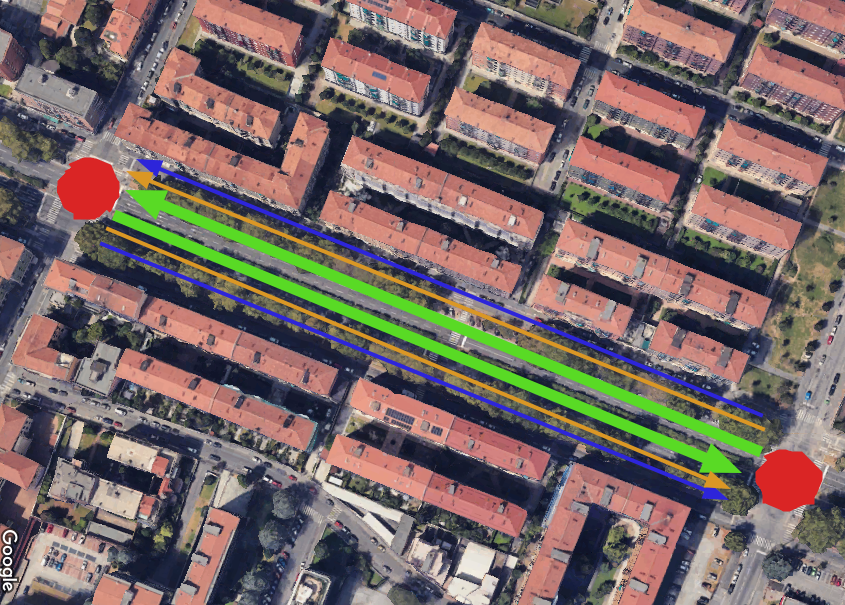
\includegraphics[width=0.75\linewidth]{figures/multigraph-is-better-than-nothing.png}
    \caption{A complex intersection pair which is connected with more different roads (Viale Zara. Milan. Italy). In \textit{green} the main lanes, in \textit{blue} the side lanes, in \textit{orange} the tramway. Source: Google Maps (2025)}
    \label{fig:multigraph-is-better-than-nothing}
\end{figure}

\begin{figure}[h]
    \centering
    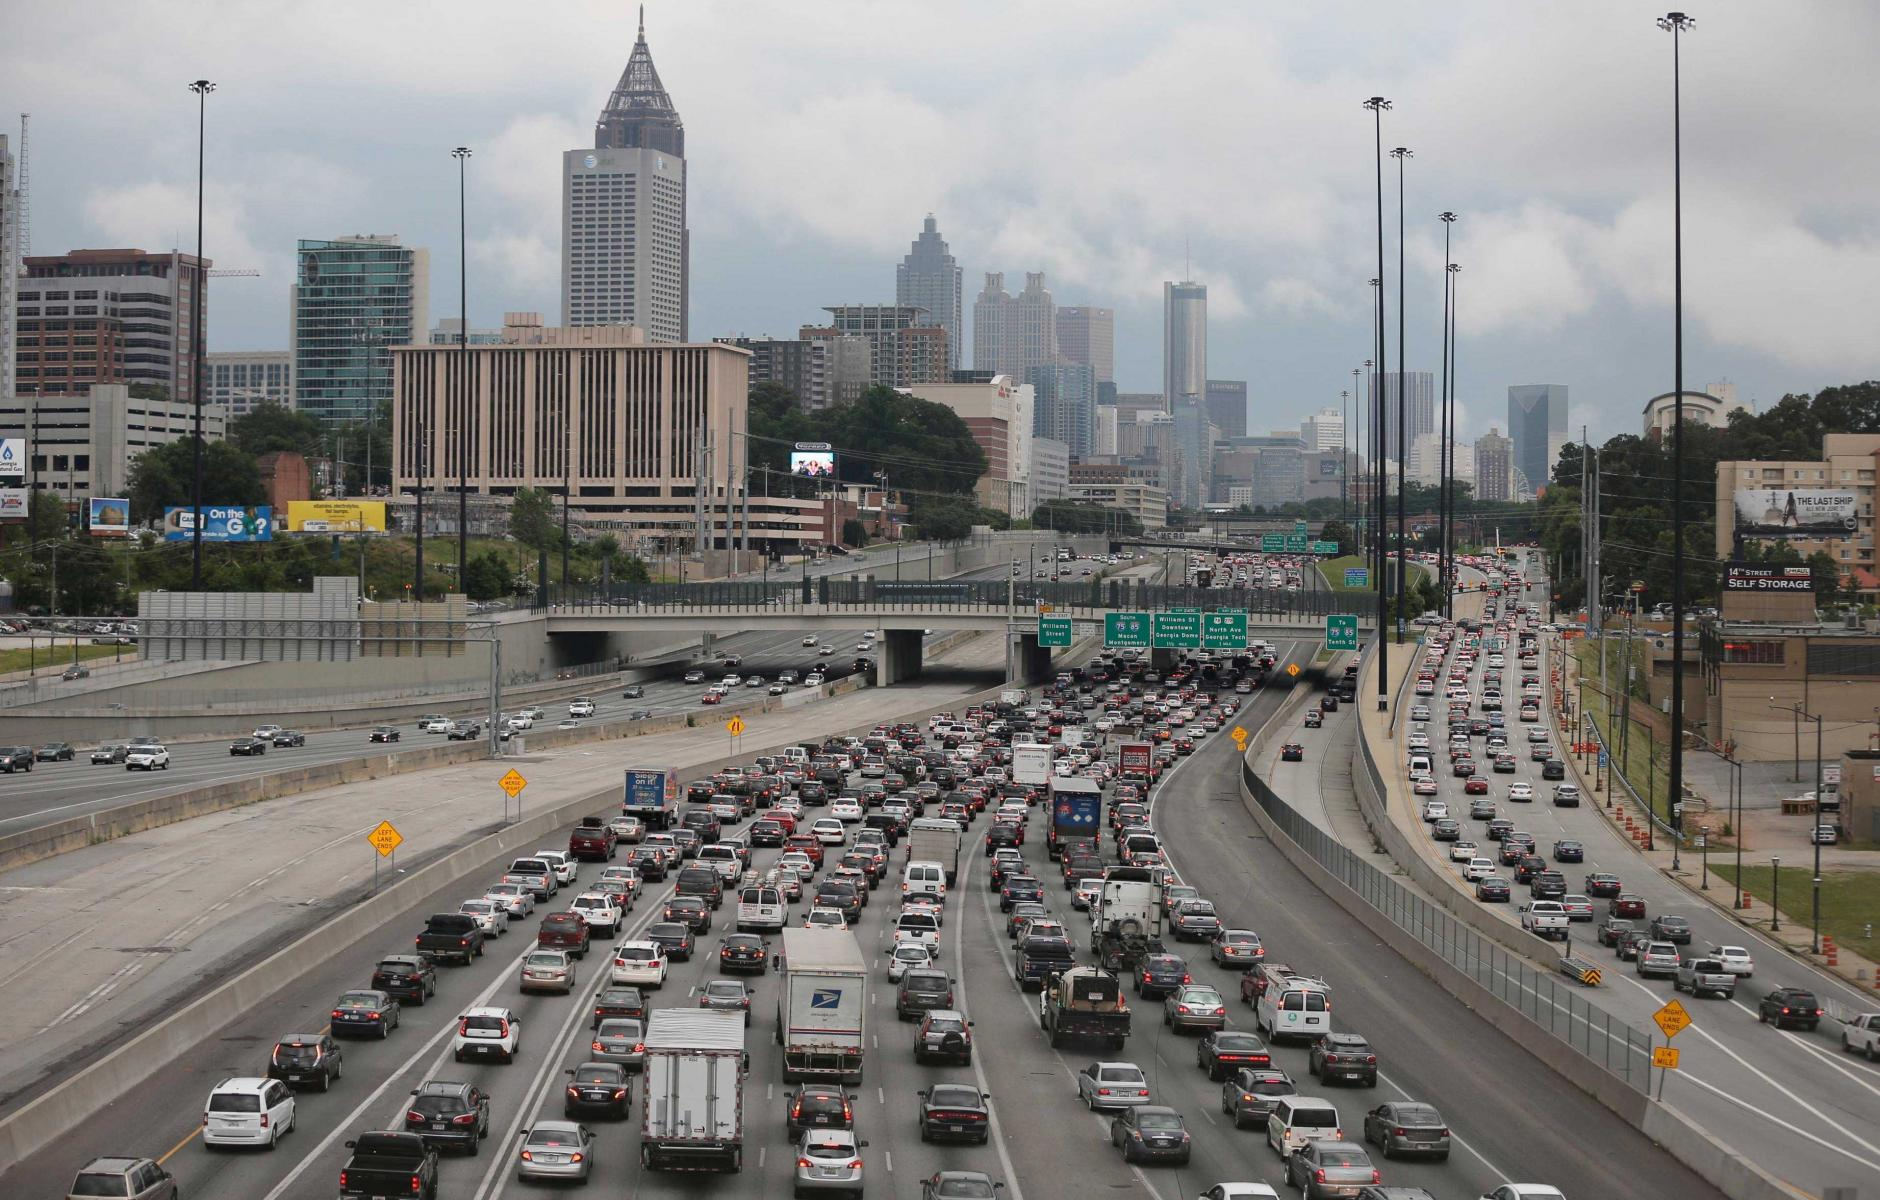
\includegraphics[width=0.75\linewidth]{figures/atlanta-georgia-freeway.jpg}
    \caption{A view of Atlanta Freeway, Georgia. Source: \href{https://www.cnu.org/publicsquare/2017/08/03/why-urban-freeway-expansion-futile}{cnu.org}}
    \label{fig:atlanta-georgia-freeway}
\end{figure}

\begin{figure}[h]
    \centering
    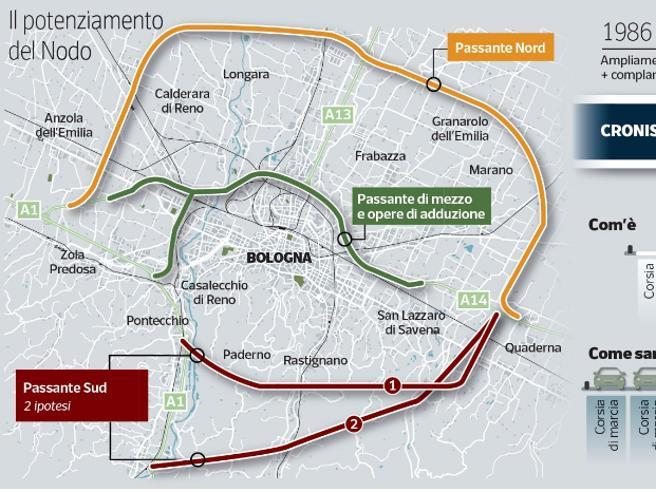
\includegraphics[width=0.75\linewidth]{figures/bologna-bypass.jpg}
    \caption{Highlight of alternatives for the Bologna node bypass. Source: Corriere della Sera}
    \label{fig:bologna-bypass}
\end{figure}

\begin{figure}[h]
    \centering
    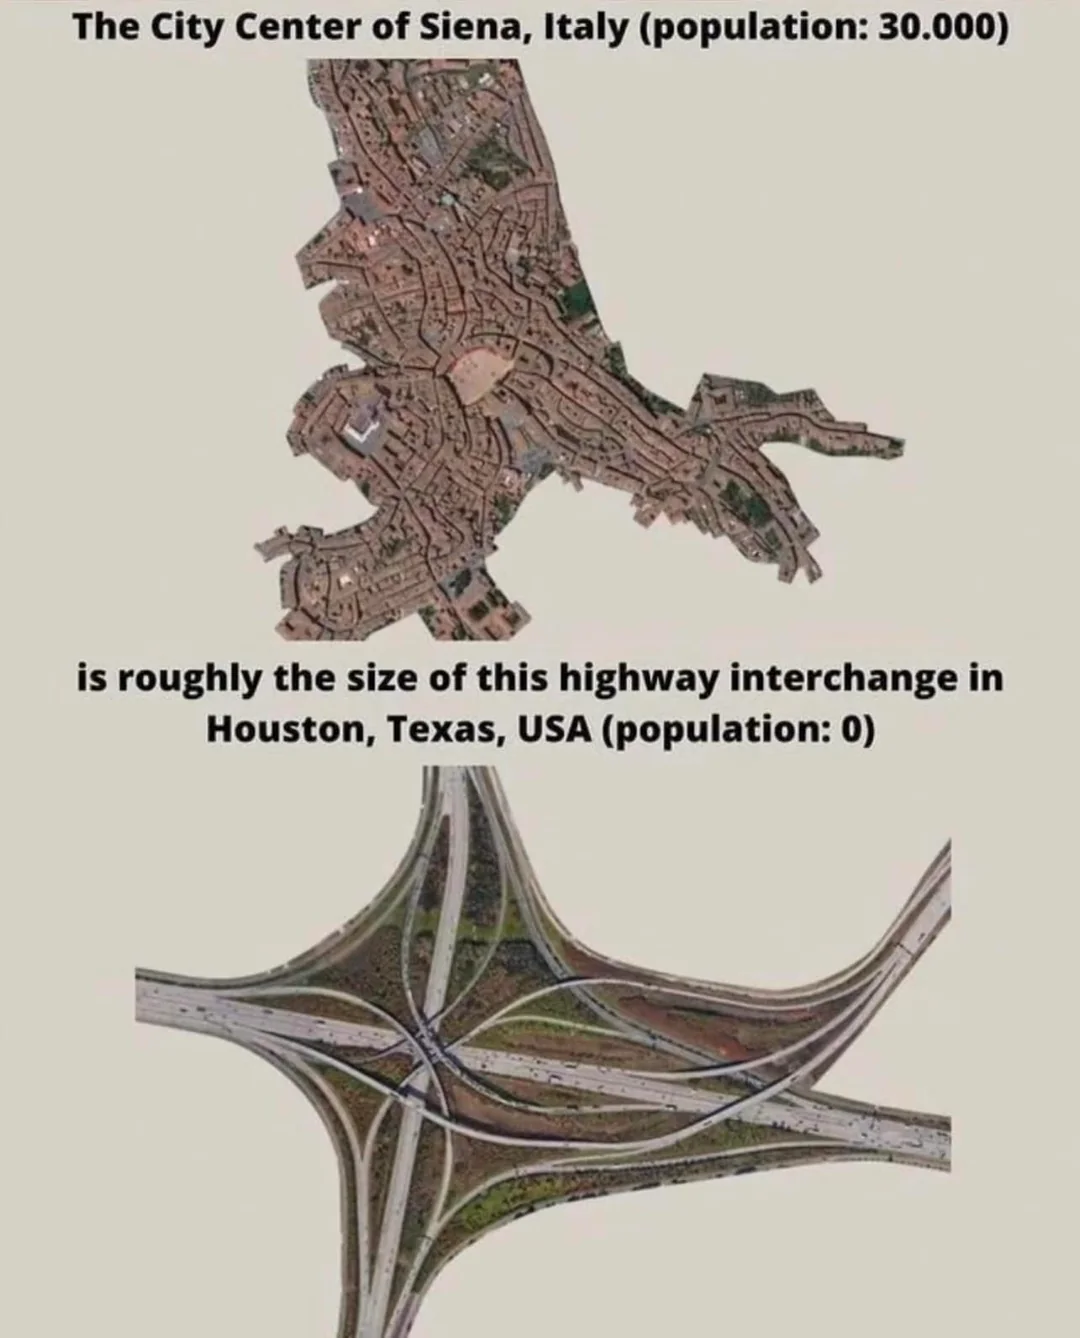
\includegraphics[width=0.75\linewidth]{figures/houston-interchange-siena.png}
    \caption{Comparison between a cloverleaf in Houston, USA, and the city center of Siena, Italy. Source: \href{https://www.reddit.com/r/geography/comments/193ryy5/siena_compared_to_highway_interchange_in_houston/}{r/geography}}
    \label{fig:houston-interchange-siena}
\end{figure}

\begin{figure}[h]
    \centering
    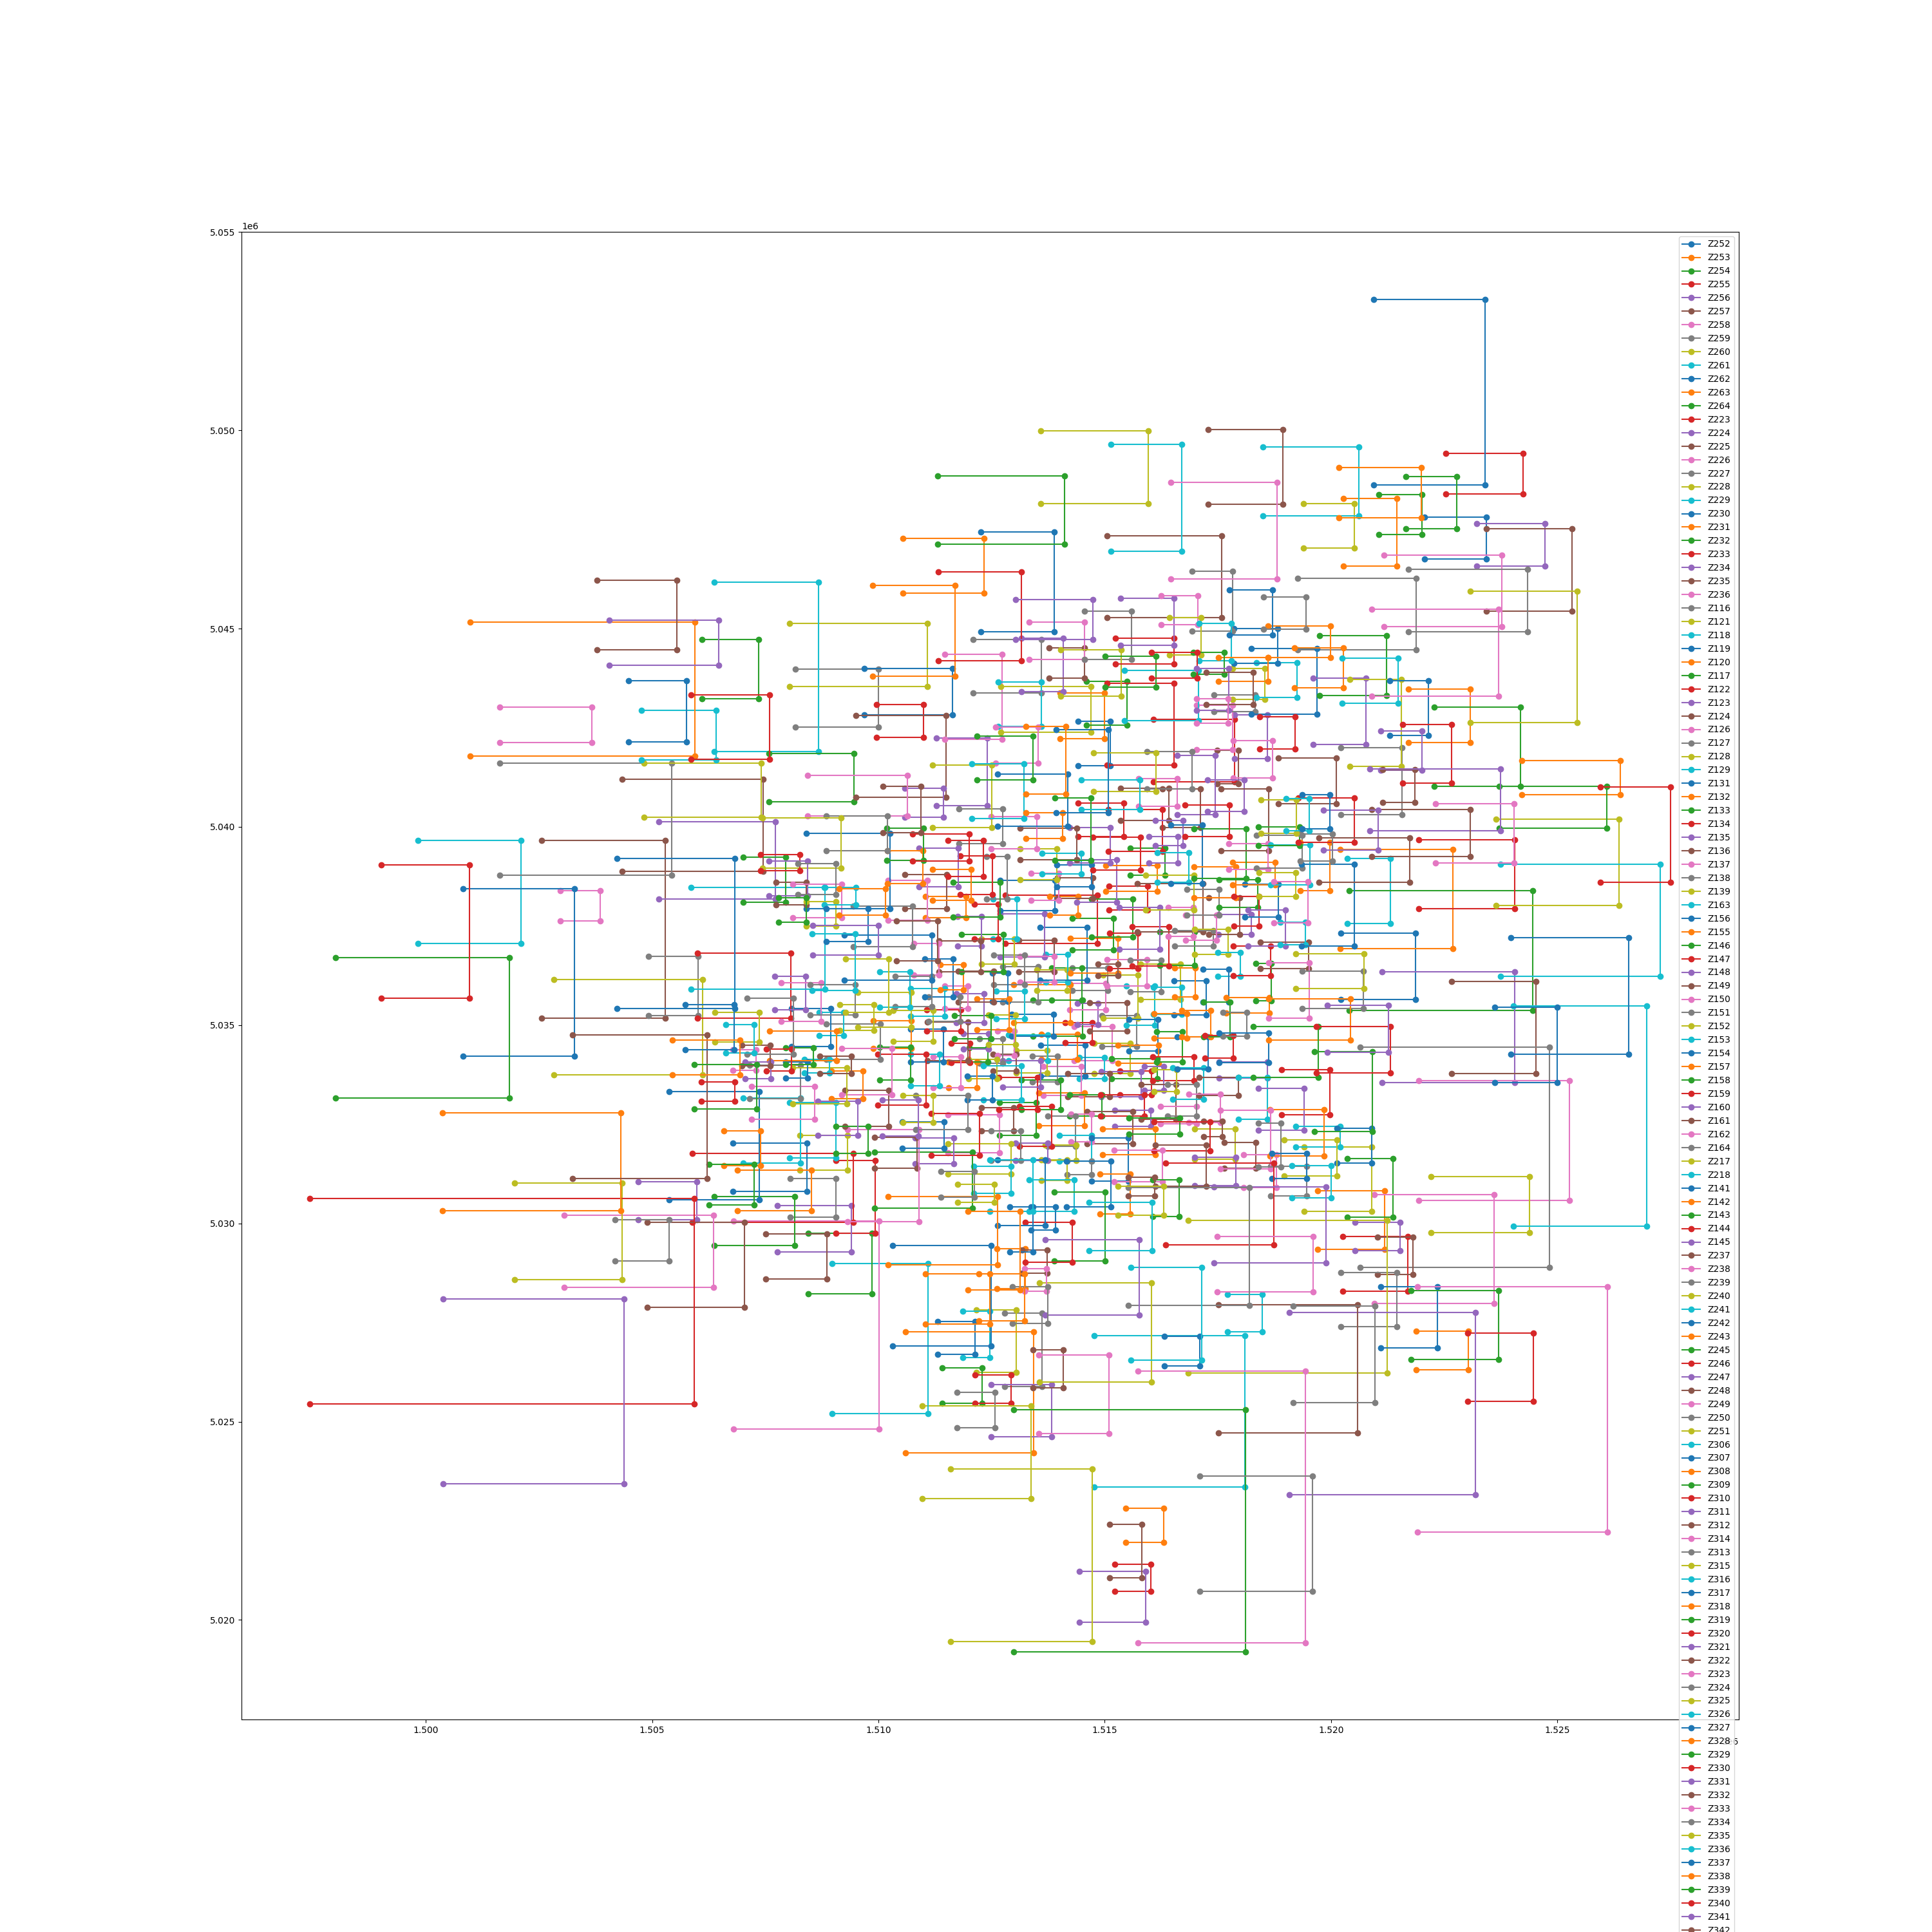
\includegraphics[width=0.75\linewidth]{figures/ODZones.Show.Milano2010.png}
    \caption{OD Zones used within the 2010 Milano AMAT model}
    \label{fig:odzones-milano-2010}
\end{figure}

\begin{figure}[h]
    \centering
    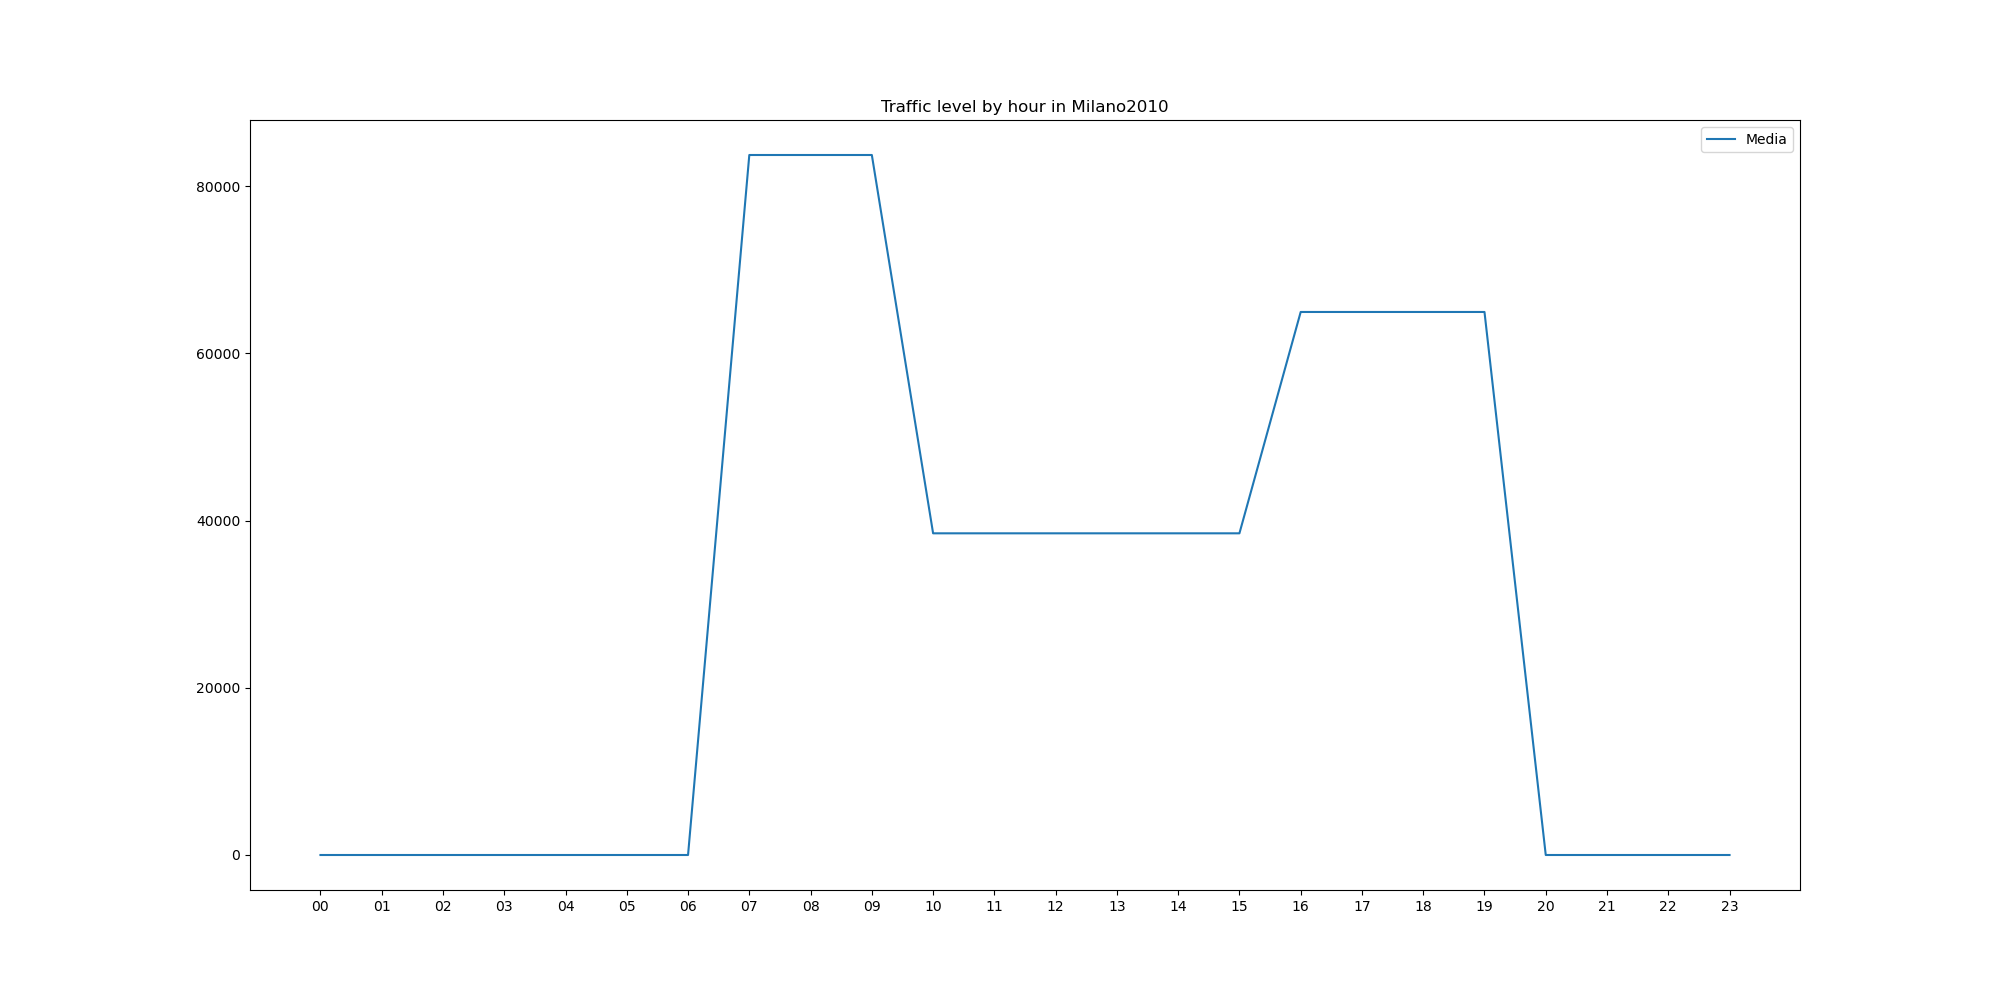
\includegraphics[width=0.75\linewidth]{figures/ODGraph.Mean.Milano2010.png}
    \caption{Traffic levels from OD Matrix of Milan in 2010}
    \label{fig:odmatrix-milano-2010}
\end{figure}

\begin{figure}[h]
    \centering
    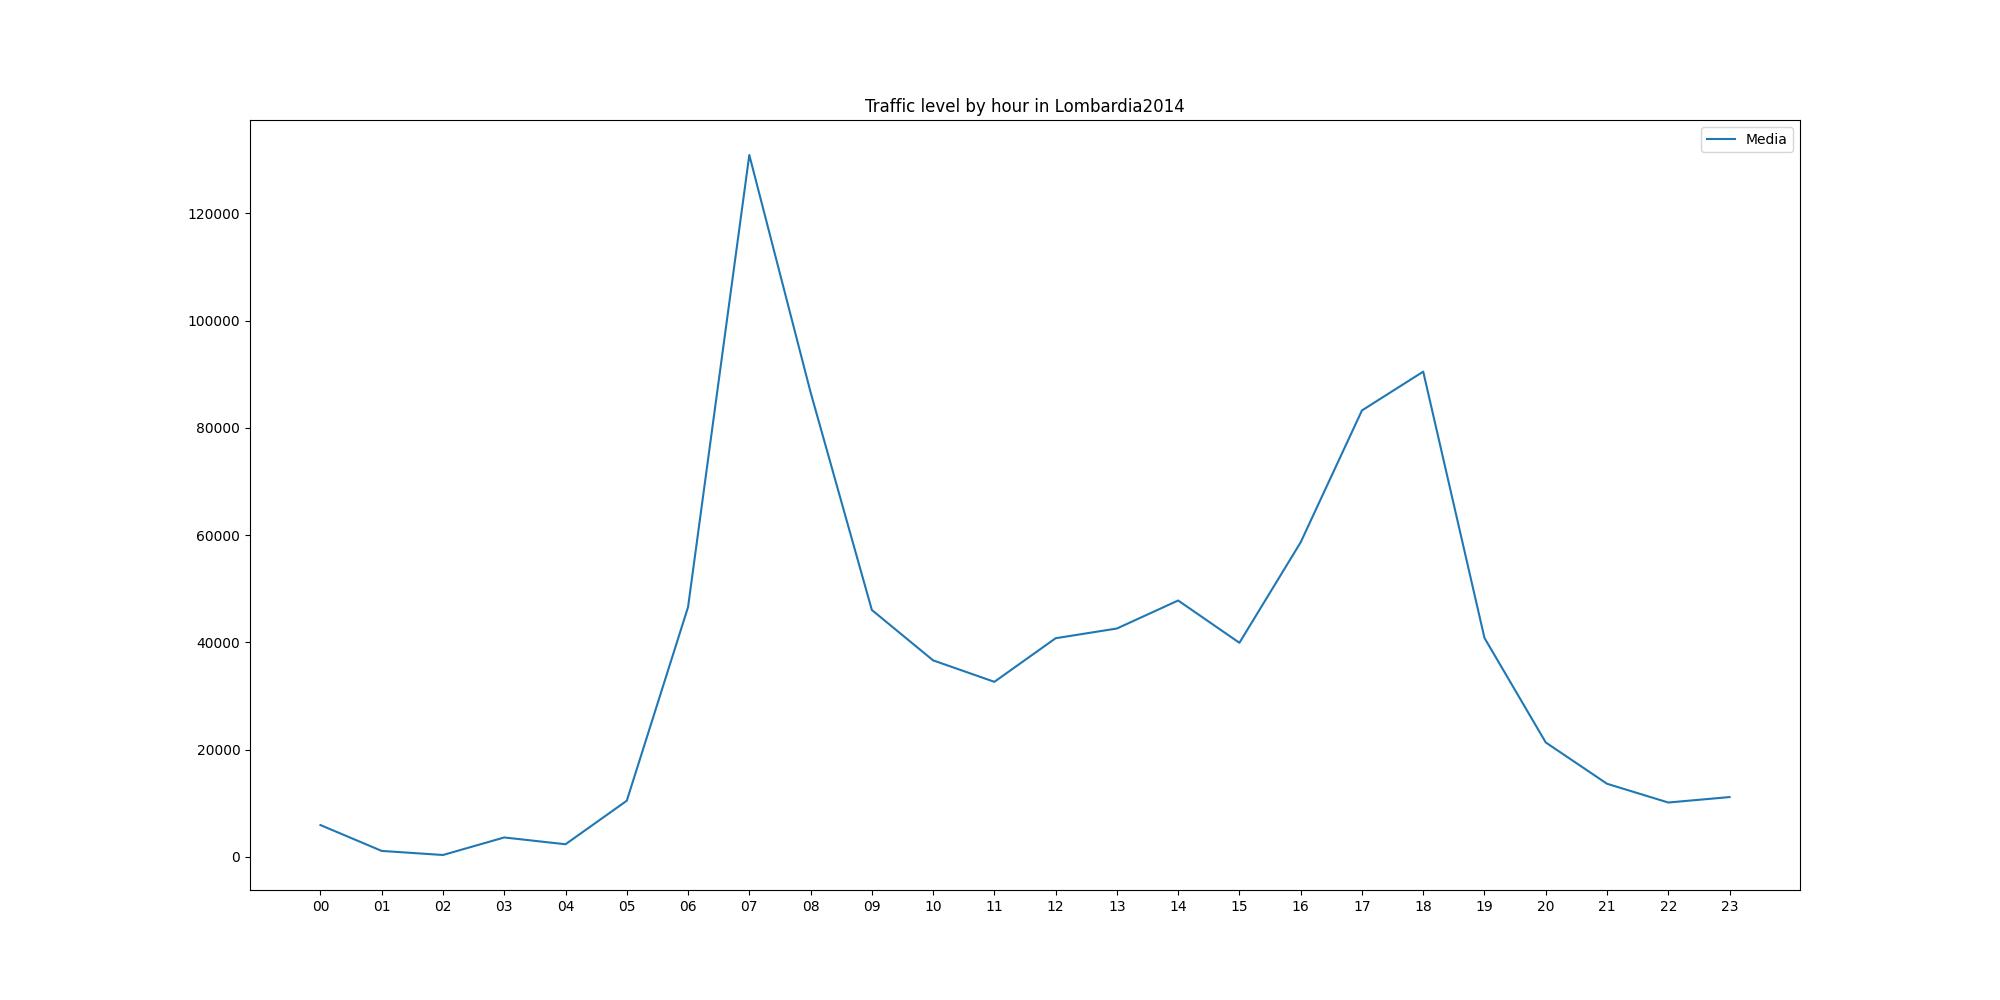
\includegraphics[width=0.75\linewidth]{figures/ODGraph.Mean.Lombardia2014.png}
    \caption{Traffic levels from OD Matrix of Lombardy in 2014}
    \label{fig:odmatrix-lombardy-2014}
\end{figure}

    
    \printbibliography
\end{document}
